\documentclass[12pt, a4paper]{article}

\usepackage[english]{babel}
\usepackage[utf8]{inputenc}
\usepackage{hyperref, bookmark}
\usepackage{graphicx}
\usepackage{fancyhdr}
\usepackage{mathtools}

% set images
\usepackage{float}

% pseudocode
\usepackage{algorithm}
\usepackage{algpseudocode}

\usepackage[left=2cm,right=2cm,top=2cm,bottom=2cm]{geometry}

% Images next to each other
\usepackage{subfig}

% citing
\usepackage[square,numbers]{natbib}
\bibliographystyle{dinat}

% general page design
\pagestyle{fancy}
\fancyhf{}
\lhead{Bachelorthesis}
\rhead{Universität Hildesheim}
\rfoot{\thepage}

% front page
\title{\LARGE Bachelorthesis\\\large Comparing different state-of-the-art solutions for image prediction using time-series analysis}
\author{ Sören Dittrich\\
	\texttt{\href{mailto:soeren.dittrich@uni-hildesheim.de}{soeren.dittrich@uni-hildesheim.de}}
}
\date{September 2020}

% start of document
\begin{document}
 \bibliographystyle{alphadin}
 
 % Abstract
 \begin{titlepage}
  \maketitle
  \thispagestyle{empty}
  \begin{abstract}\noindent 
   % Abstract
The thesis will compare different state-of-the-art solutions for image-/video-prediction \ref{subsection::imageprediction}.
The main module of those solutions, which is the core aspect of this work, is the LSTM (Long short-term memory) \ref{subsection::lstm}.
This module was invented by Hochreiter and Schmidhuber  \cite{Hochreiter1997} in 1997 and is used heavily in the field of image-\& video-prediction since then, e.g. in Srivastava et al. 
\cite{Srivastava2015}.
During the time the module got many different add-ons and changes, which are described in different papers (\cite{Patraucean2015}, \cite{Lotter2016}, \cite{Wang2017}, \cite{Wang2018} and many 
more.). 
This thesis is giving a comprehensive overview over a selection of image-/video-prediction algorithms and experimenting if the more advanced solution PredRNN \cite{Wang2017} is able to outperform the standard ConvLSTM module. This is done, by implementing
three different state-of-the-art solutions for image-/video-prediction (\cite{Shi2015}, \cite{Patraucean2015} and \cite{Lotter2016}).
All of them use a ConvLSTM solution as recurrent sub-module, which is changed during the experiments
with the more advanced solution PredRNN \cite{Wang2017}, to see if the usage of a more advanced recurrent sub-module will increase the accuracy.\\
The algorithms are therefore re-implemented in PyTorch \cite{Paszke2019}.
  \end{abstract}
 \end{titlepage}
 
 % Table of contents
 \tableofcontents
 \newpage
 
 % question
 % section
\section*{Scientific questions}
 \begin{enumerate}
  \item What different types of image prediction architectures exist?
  \item How important is the choice of the recurrent module for the runtime and performance of the algorithm?
 \end{enumerate}
 \newpage
 
 % introduction
 % section
\section{Introduction} \label{section::introduction}
 The thesis will compare different state-of-the-art solutions for image prediction \ref{subsection::imageprediction}.
 The main module, which is a core aspect of this work, is the LSTM (Long short-term memory). \ref{subsection::convlstm}.
 This module was invented by Hochreiter and Schmidhuber  \cite{Hochreiter1997} in 1997 and is used heavily in the field of image prediction since then, e.g. in Srivastave et. al. 
 \cite{Srivastava2015}.
 During the time the module got many different add-ons and changes, which are described in different papers (\cite{Patraucean2015}, \cite{Lotter2016}, \cite{Wang2017}, \cite{Wang2018} and many 
 more.). This work is implementing one specific network architecture (PredNet \cite{Lotter2016}).
 It uses the Shi et. al. \glqq standard\grqq ConvLSTM \cite{Shi2015} as recurrent sub-module, which is changed during the experiments
 with other (more advanced) solutions. The PredNet algorithm is re-implemented in PyTorch \cite{Paszke2019}, as well as the \glqq standard\grqq ConvLSTM and PredRNN.
 Practical experiments are performed on the PredNet using the \glqq standard\grqq ConvLSTM
 and on PredNet using PredRNN instead.
 
 % subsection
 \subsection{Deep Learning} \label{subsection::deeplearning}
 
 % subsection
 \subsection{Image Prediction} \label{subsection::imageprediction}
  Image prediction is a field inside machine learning, where the key is to predict future images, given a sequence of image. The image sequence $X$ is of length $n$, ($x_0, \ldots, x_{n-1}$).
  One possible use-case is the one-frame prediction, where one predicts $x_n$, given the the sequence $X$. Another common use-case is multi-frame prediction, where the key is to predict $t$ many
  frames into the future. This is often performed using sequence-to-sequence learning \cite{Sutskever2014}. Obviously the first frames look much better then the last frames, as ground-truth is 
  missing, and the predicted frames are approximated, which means they contain a certain level of error.

 % subsection
 \subsection{Autoencoder} \label{subsection::autoencoder}

 % subsection
 \subsection{RNN} \label{subsection::rnn}
  RNN (Recurrent neural network)
 
 % subsection
 \subsection{LSTM} \label{subsection::lstm}
  LSTM (Long Short-term Memory) \cite{Hochreiter1997} is a form of RNN, which avoids a critical problem of standard RNN: Saving \textbf{Long-term dependencies} \cite{Goodfellow2016}.
  The architecture consists of different submodules, an inpute-gate, forget-gate, cell-state and output-gate.
  \begin{equation}
   i_t = \sigma(w_{x_i}x_t + w_{h_i}h_{t-1} + w_{c_i}c_{t-1} + b_i)
  \end{equation}
  \begin{equation}
   f_t = \sigma(w_{x_f}x_t + w_{h_f}h_{t-1} + w_{c_f}c_{t-1} + b_f)
  \end{equation}
  \begin{equation}
   c_t = f_tc_{t-1} + i_ttanh(w_{x_c}x_t + w_{h_c}h_{t-1} + b_c)
  \end{equation}
  \begin{equation}
   o_t = \sigma(w_{x_o}x_t + w_{h_o}h_{t-1} + w_{c_o}c_t + b_o)
  \end{equation}
  \begin{equation}
   h_t = o_ttanh(c_t)
  \end{equation}
  $w$ is the weight of the layer, $\sigma$ the sigmoid function, $b$ the layer bias. $h_t$ is the output, in RNN's
  the output is often denoted as hidden.
  \begin{figure}[H]
   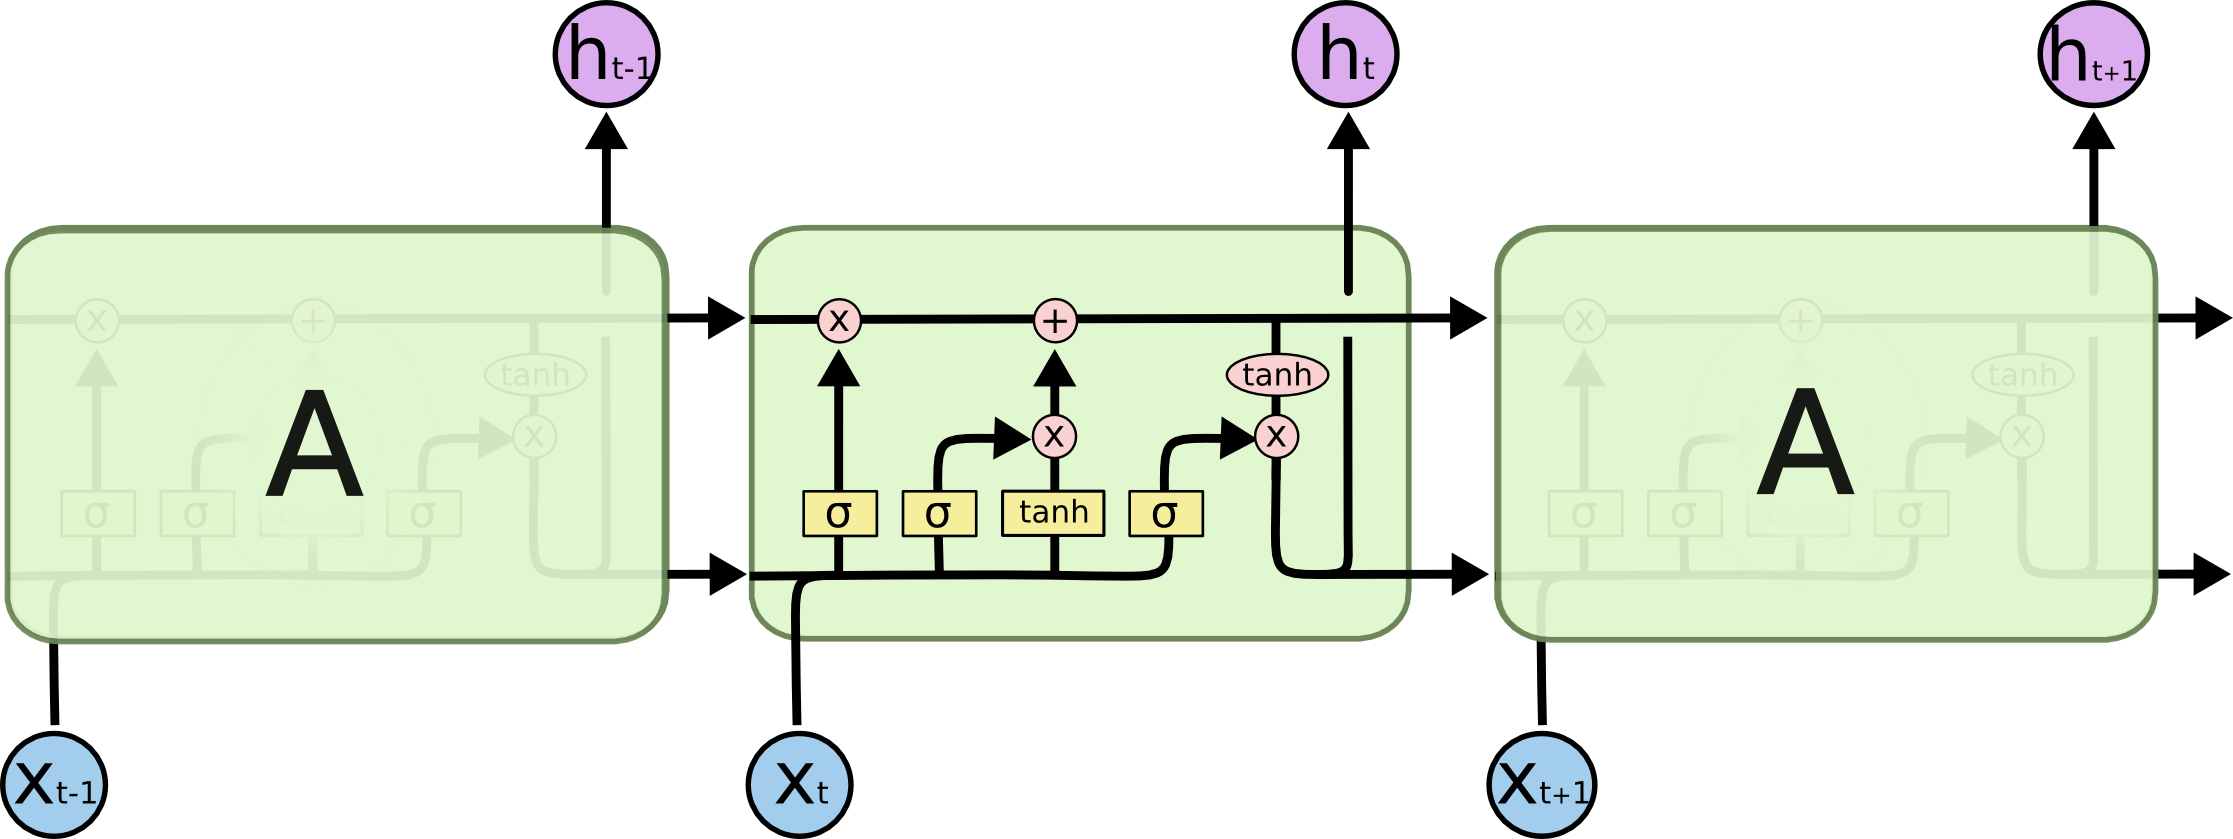
\includegraphics[width=0.6\textwidth]{../Images/lstm_chain.png}
   \centering
   \caption{LSTM Architecture \citep{Olah2015}}
   \label{fig:lstm_architecture}
  \end{figure}
 
 % subsection
 \subsection{ConvLSTM} \label{subsection::convlstm}
  The convolutional LSTM, invented by Shi et. al. \cite{Shi2015} is a LSTM using convolutional layer instead of fully connected ones. Therefore the formulas looks very similar to the ones in    
  section~\ref{subsection::lstm}.
  \begin{equation}
   i_t = \sigma(x_t \ast w_{x_i} + h_{t-1} \ast w_{h_i} + w_{i_b})
  \end{equation}
  \begin{equation}
   f_t = \sigma(x_t \ast w_{x_f} + h_{t-1} \ast w_{h_f} + w_{f_b})
  \end{equation}
  \begin{equation}
   \tilde{c_t} = tanh(x_t \ast w_{x_{\tilde{c}}} + h_{t-1} \ast w_{h_{\tilde{c}}} + w_{c_{\tilde{b}}})
  \end{equation}
  \begin{equation}
   c_t = \tilde{c_t} \odot i_t + c_{t-1} \odot f_t
  \end{equation}
  \begin{equation}
   o_t = \sigma(x_t \ast w_{x_o} + h_{t-1} \ast w_{h_o} + w_{o_b})
  \end{equation}
  \begin{equation}
   h_t = o_t \odot tanh(c_t)
  \end{equation}
  $\ast$ is the commonly used sign for the convolution operation.\\
  $\odot$ is the hadamard product (point-wise multiplication).
  
 % subsection
 \subsection{PyTorch} \label{subsection::pytorch}

 % related work
 % section
\section{Image Prediction Architectures} 
 % subsection
 \subsection{LSTM Autoencoder}
  % page 1
  \begin{frame}
   \frametitle{LSTM Autoencoder}
   
   \begin{itemize}
    \item<1-> \glqq Unsupervised Learning of Video Representations using LSTMs\grqq by Srivastava et. al. \cite{Srivastava2015}
    \item<2-> Using the standard LSTM from Hochreiter \& Schmidhuber \cite{Hochreiter1997}
    \item<3-> Autoencoder architecture
    \item<4-> Useful for future image prediction \& image reconstruction
    \item<5-> Typical baseline for newer, more advanced algorithms
   \end{itemize}
   
  \end{frame}
  % page 2
  \begin{frame}
   \frametitle{LSTM Autoencoder}
   
   \begin{figure}[H]
    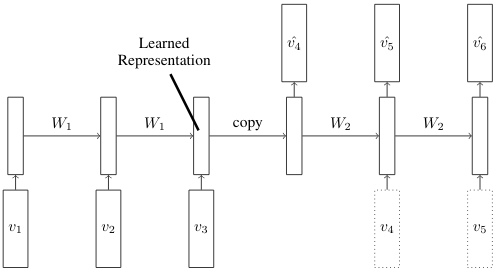
\includegraphics[width=0.7\textwidth]{../Images/srivastava.png}
    \centering
    \caption{Future image prediction model \citep{Srivastava2015}}
    \label{fig:lstm_architecture}
   \end{figure}
  
  \end{frame}
  % page 3
  \begin{frame}
   \frametitle{LSTM Autoencoder}  
  
   \begin{figure}[H]
    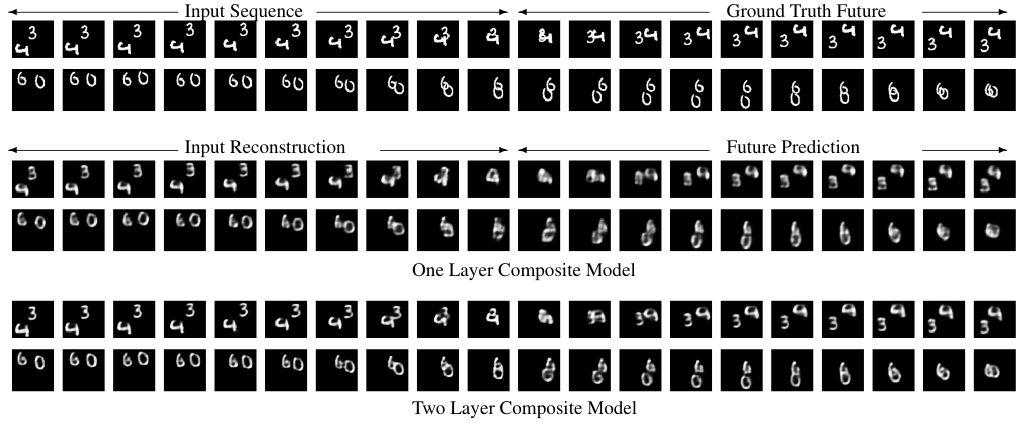
\includegraphics[width=0.7\textwidth]{../Images/srivastava_results_mnist.png}
    \centering
    \caption{Results of MovingMNIST experiment \citep{Srivastava2015}}
    \label{fig:lstm_results_mnist}
   \end{figure}
  
  \end{frame}
 
 % subsection
 \subsection{ConvLSTM Autoencoder}
  % page 1
  \begin{frame}
   \frametitle{ConvLSTM Autoencoder}
   
   \begin{itemize}
    \item<1-> \glqq Convolutional LSTM Network: A Machine Learning Approach for Precipitation Nowcasting\grqq by Shi et. al. \citep{Shi2015}
    \item<2-> Similar to LSTM Autoencoder, but uses ConvLSTM instead
    \item<3-> Outperforms the LSTM Autoencoder
   \end{itemize}
   
  \end{frame}
  % page 2
  \begin{frame}
   \frametitle{ConvLSTM Autoencoder}
   
   \begin{figure}[H]
    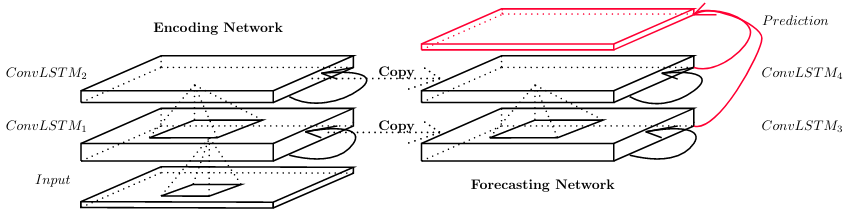
\includegraphics[width=1.0\textwidth]{../Images/shi.png}
    \centering
    \caption{Future image prediction model \citep{Shi2015}}
    \label{fig:convlstm_architecture}
   \end{figure}
  
  \end{frame}
  % page 3
  \begin{frame}
   \frametitle{ConvLSTM Autoencoder}
   
   \begin{figure}[H]
    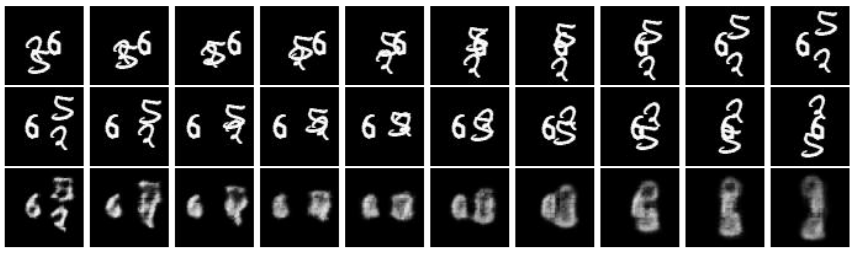
\includegraphics[width=0.7\textwidth]{../Images/shi_results_mnist.png}
    \centering
    \caption{Results of MovingMNIST experiment \citep{Srivastava2015}}
    \label{fig:lstm_architecture}
   \end{figure}  
  
  \end{frame}
 
 % subsection
 \subsection{Spatio-temporal Video Autoencoder}
  % page 1
  \begin{frame}
   \frametitle{Spatio-temporal Video Autoencoder}
   
   \begin{itemize}
    \item<1-> \glqq Spatio-Temporal Video Autoencoder With Differentiable Memory \grqq by Patraucean et. al. \cite{Patraucean2015}
    \item<2->
   \end{itemize}
   
  \end{frame}
  % page 2
  \begin{frame}
   \frametitle{Spatio-temporal Video Autoencoder}
   
   \begin{figure}[H]
    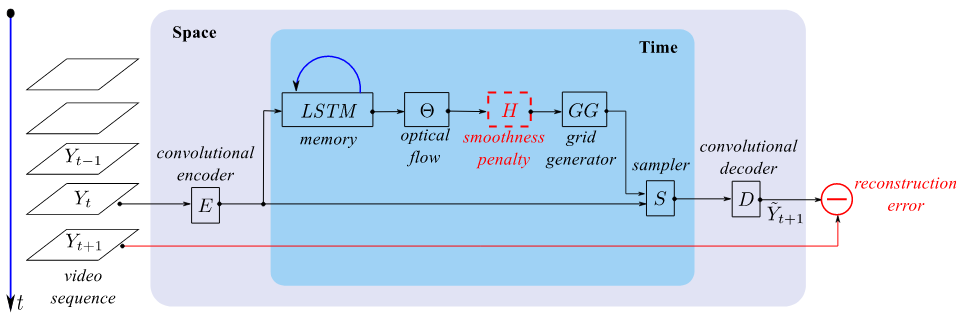
\includegraphics[width=1.0\textwidth]{../Images/patraucean.png}
    \centering
    \caption{Spatio-temporal Video Autoencoder Architecture \citep{Patraucean2015}}
    \label{fig:spatiotemp_architecture}
   \end{figure}
  
  \end{frame}
  % page 3
  \begin{frame}
   \frametitle{Spatio-temporal Video Autoencoder}  
  
   \begin{figure}[H]
    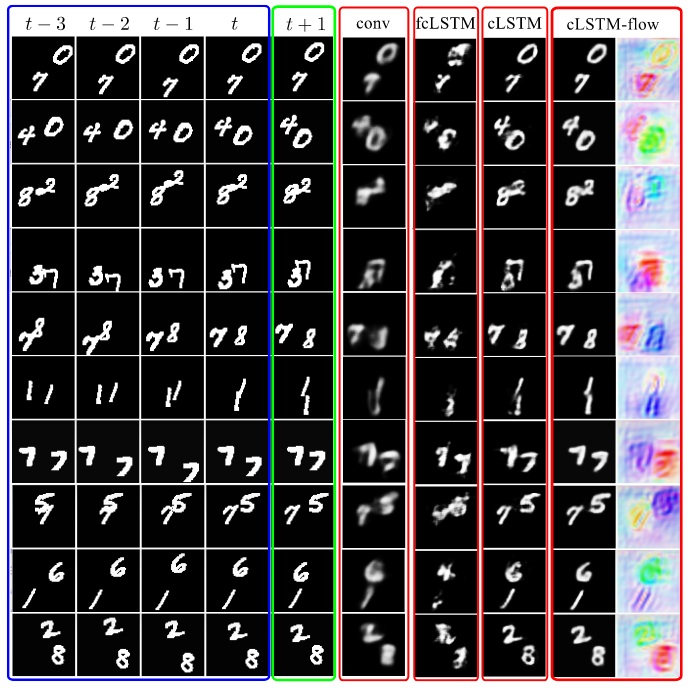
\includegraphics[width=0.55\textwidth]{../Images/patraucean_results_mnist.png}
    \centering
    \caption{Results of MovingMNIST experiment \citep{Patraucean2015}}
    \label{fig:lstm_architecture}
   \end{figure}  
  
  \end{frame}
 
 % subsection
 \subsection{PredNet}
  \begin{frame}
   \frametitle{PredNet}
   
  \end{frame}
  
 % subsection
 \subsection{PredRNN}
  \begin{frame}
   \frametitle{PredRNN}  
  
  \end{frame}

 
 % algorithm
 % section
\section{Implementation}
  

 
 % usage
  

 
 % training
 % section
\section{Training} \label{section::training}
The training section will cover the aspects of different training types.
 
 % experiments
 % section
\section{Experiments} \label{section::experiments}
 This section describes the experiments performed on the three networks and the results those experiments gave. The experiments were performed, to see if the 
 implemented networks are able to perform better, when changing the recurrent sub-module with a more advanced recurrent module. The sections starts with the  
 description of the experimental setup, followed by the experimental results.
 
 % subsection
 \subsection{Experimental Setup}
  The experiments were performed on three different datasets. First of all, I started using a synthetic dataset. This has the advantage of having full knowledge
  about the underlying structure of the data and that one has, in theory, an infinite amount of data for training and testing. This is also a very common approach
  and performed in all papers, compared in section~\ref{section::related}.
  For the synthetic dataset I used MovingMNIST, which is a dataset created using handwritten digits from the famous handwritten dataset MNIST
  \cite{LeCun1998}. The idea is to use a pre-defined number of digits, which are spawned at a random position inside a given frame. Those digits are then moved 
  through the frame, given a velocity and momentum. If a digit will touch the boundary of the frame, the digit will bounce back.\\
  The other two used datasets are real datasets\footnote{Camera images or videos from the real world.}.
  The first one is KTH \cite{Schuldt2004}, an action recognition dataset, which consists of videos where people
  do different actions, such as hand waving, running and jogging. The second one is Kitti \cite{Geiger2013}, which is an autonomous driving dataset, where
  the authors drove a car through different areas in Karlsruhe, Germany. For example through residential areas and the city.\\\\
  I pre-processed MovingMNIST, to have a frame size of $(1 \times 64 \times 64)$, two digits per frame and ten frames per sequence.
  The training set consists of $10000$ sequences and the test set of $3000$ sequences.\\
  KTH was pre-processed to gray-scaled images and cropped to the frame size $(1 \times 80 \times 60)$.\\
  Kitti was also cropped to a specific frame size $(3 \times 160 \times 128)$.\\\\
  To have a valid comparison, I decided to fix the amount of epochs and iterations per dataset, as well as all frames are normalized and having MSE as the
  error function for training and testing.\\
  For MovingMNIST, I used one epoch with $5000$ iterations, for KTH $20$ epochs with $500$ iterations per epoch and for Kitti $50$ epochs with $500$ iterations
  per epoch. The values for MovingMNIST are inspired by Elsayed et al. \cite{Elsayed2018}, where they develop a novel ConvLSTM module for PredNet and train
  PredNet on the MovingMNIST dataset (Which is not done by the PredNet authors.). The values for KTH and Kitti are inspired by Lotter et al. \cite{Lotter2016}.
  In the PredNet paper the authors use $150$ epochs with $500$ iterations per epoch to train PredNet on Kitti dataset, but I reduced the amount of epochs to
  $50$ because the training would otherwise take more then $20$ hours, which was not applicable for me. Because KTH is a more \glqq simple\grqq dataset (Only 
  objects in the scenery are moving, not the scenery as in Kitti.), I artificially chose $20$ as the amount of epochs.\\\\
  I used Adam \cite{Kingma2015} as optimizer for all networks, always with the same learning rate, of $0.001$, and the same learning rate scheduler (Dividing the 
  learning rate by factor ten after $50$\% of epochs.), even tho 
  Patraucean et al. \cite{Patraucean2015} are using RMSProp \cite{Ruder2016}, in their paper, as optimizer and a different learning rate scheduler.
  The values are used by Lotter et al. \cite{Lotter2016} for PredNet, so I chose them as the hyperparameter for this experiment.
  But the idea behind those fixed values is simply, that all networks get the same amount of data with the same optimizer, the same learning rate scheduler 
  without any unfair advantage, because the experiment is the comparison of the network using two different recurrent submodules. So both implementations
  have the same starting point, even tho the hyperparameter might not be the best for the network to reach the best performance.
  The network parameters, e.g. the depth of the autoencoder, were chosen from the corresponding papers.\\\\
  In general there would be so many different additions to add to the experiments, such as early stopping, random restarts, grid- or random-
  search, the usage of dropout and trying different optimizer and learning rate scheduler, but all those additions take plenty of computing time, which was not 
  applicable for me and the scope of this thesis.\\
  
  
 % subsection
 \subsection{Experimental Results}
  This section is divided into the three different datasets, but all those subsections is structured the same way. It starts by comparing the amount of paramters
  for the dataset, because the amount of parameters is directly correlated to the computing time, the network needs for training and testing. It then shows
  some training graphs, to proove that the networks really learned something, followed by examples of the testing output at the end and a table of mean MSE error.
  The number of parameters directly correlates to the performance\footnote{In computer science, the performance directly correlates with the computing time.}, 
  therefore is a smaller amount always better, because the network will train faster and is also faster at test time. A tree graph of the performed experiments
  can be found in the appendix~\ref{section::appendix}.
  
  % subsubsection
  \subsubsection{MovingMNIST}
   \begin{table}[H]
    \begin{center}
     \begin{tabular}{| l | l | l |}\hline
      \textbf{Model} & \textbf{ConvLSTM} & \textbf{PredRNN} \\\hline
      Autoencoder (Depth $2$) & $537.411$ & $773.018$ \\\hline
      PredNet & $6.909.818$ & $12.421.090$ \\\hline
      Spatiotemp & $1.001.324$ & $1.415.639$ \\\hline
     \end{tabular}
    \end{center}
    \caption{Number of trainable parameter for MovingMNIST.}
   \end{table}\noindent
   We can clearly see, that the networks using PredRNN, due to it's more complex architecture, has at least $~1.41$ times the amount of parameters. In the worst
   case, here for PredNet (Because PredNet has the PredRNN module in every layer.), the value is $~1.8$. This results show, that the networks using PredRNN
   should perform better in the test to be the superior architecture, because otherwise they don't have any advantage to the architecture using ConvLSTM.
   \begin{figure}[H]
    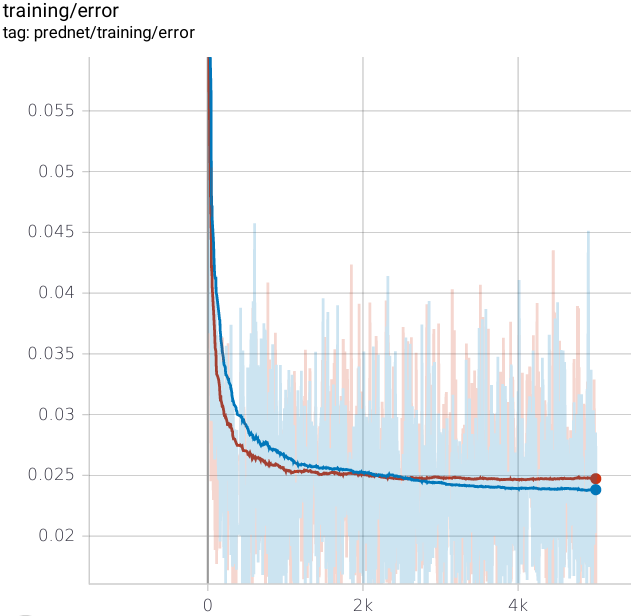
\includegraphics[width=0.55\textwidth]{../Images/prednet_mnist_training.png}
    \centering
    \caption{Training PredNet with ConvLSTM (blue) and PredRNN (red) on MovingMNIST.}
    \label{fig:prednet_mnist_training}
   \end{figure}\noindent
   \begin{figure}[H]
   \centering
   \subfloat[Ground truth]{{
\includegraphics[width=0.6\textwidth]{../Images/prednet_mnist_groundtruth.png} }} 
   \qquad
   \subfloat[ConvLSTM]{{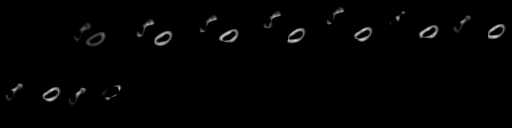
\includegraphics[width=0.6\textwidth]{../Images/prednet_mnist_convlstm_prediction.png} }} 
   \qquad
   \subfloat[PredRNN (vanished)]{{
\includegraphics[width=0.6\textwidth]{../Images/prednet_mnist_predrnn_prediction.png} }}
   \caption{Test results for PredNet on MovingMNIST.}
   \label{figure::prednet_mnist_results}
  \end{figure}\noindent
  Here one can see a problem, that was always present during training. The values for MovingMNIST were vanishing very fast, which often resulted in empty images,
  for ConvLSTM and PredRNN. This is due to the fact, that PyTorch is vanishing gradients faster then Keras \cite{chollet2015}, and that Lotter et al. used 
  Matplotlib \cite{Hunter2007}, which is able to catch much smaller values then Tensorboard is (I had to multiply the values with factor ten, to even get some
  output.).
    
  This is one case of using random restarts to have a network which is not vanishing.
   \begin{table}[H]
    \begin{center}
     \begin{tabular}{| l | l | l |}\hline
      \textbf{Model} & \textbf{ConvLSTM} & \textbf{PredRNN} \\\hline
      Autoencoder (Depth $2$) & $0.027$ & $0.028$ \\\hline
      PredNet & $0.035$ & $0.041$ \\\hline
      Spatiotemp & $0.024$ & $0.022$ \\\hline
     \end{tabular}
    \end{center}
    \caption{Mean MSE for MovingMNIST.}
   \end{table}\noindent
   Those values directly show, that the change from ConvLSTM to PredRNN does not make any positive difference for any network performing the tests on MovingMNIST.
   Therefore, as written above, the network using PredRNN only consist of more parameter, so the choice should therefore tend to ConvLSTM, because it has less
   computing time and similar results.
   
  % subsubsection
  \subsubsection{KTH}
   \begin{table}[H]
    \begin{center}
     \begin{tabular}{| l | l | l |}\hline
      \textbf{Model} & \textbf{ConvLSTM} & \textbf{PredRNN} \\\hline
      Autoencoder (Depth $2$) & $542.531$ & $781.760$ \\\hline
      PredNet & $850.325$ & $1.285.730$ \\\hline
      Spatiotemp & $1.007.598$ & $1.421.913$ \\\hline
     \end{tabular}
    \end{center}
    \caption{Number of trainable parameter for KTH.}
   \end{table}\noindent
   \begin{figure}[H]
   \centering
   \subfloat[Ground truth]{{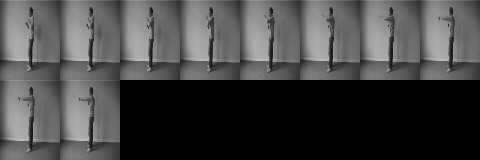
\includegraphics[width=0.6\textwidth]{../Images/prednet_kth_groundtruth.png} }} 
   \qquad
   \subfloat[ConvLSTM]{{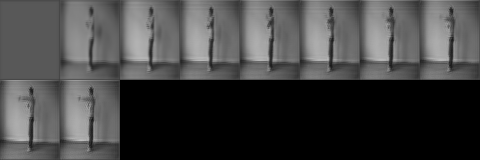
\includegraphics[width=0.6\textwidth]{../Images/prednet_kth_convlstm.png} }} 
   \qquad
   \subfloat[PredRNN]{{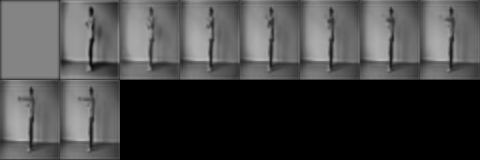
\includegraphics[width=0.6\textwidth]{../Images/prednet_kth_predrnn.png} }}
   \caption{Test results for PredNet on KTH.}
   \label{figure::prednet_kth_results}
  \end{figure}\noindent
   \begin{table}[H]
    \begin{center}
     \begin{tabular}{| l | l | l |}\hline
      \textbf{Model} & \textbf{ConvLSTM} & \textbf{PredRNN} \\\hline
      Autoencoder (Depth $2$) & $1.55e-3$ & $0.05$ (didn't converged) \\\hline
      PredNet & $1.95e-3$ & $1.93e-3$ \\\hline
      Spatiotemp & $3.1e-3$ & $0.025$ (didn't converged) \\\hline
     \end{tabular}
    \end{center}
    \caption{Mean MSE for KTH.}
   \end{table}
  
  % subsubsection
  \subsubsection{Kitti}
   \begin{table}[H]
    \begin{center}
     \begin{tabular}{| l | l | l |}\hline
      \textbf{Model} & \textbf{ConvLSTM} & \textbf{PredRNN} \\\hline
      Autoencoder (Depth $2$) & $542.531$ & $781.760$ \\\hline
      PredNet & $8.222.559$ & $12.430.626$ \\\hline
      Spatiotemp & $1.640.321$ & $2.200.641$ \\\hline
     \end{tabular}
    \end{center}
    \caption{Number of trainable parameter for Kitti.}
   \end{table}\noindent
   \begin{figure}[H]
   \centering
   \subfloat[Ground truth]{{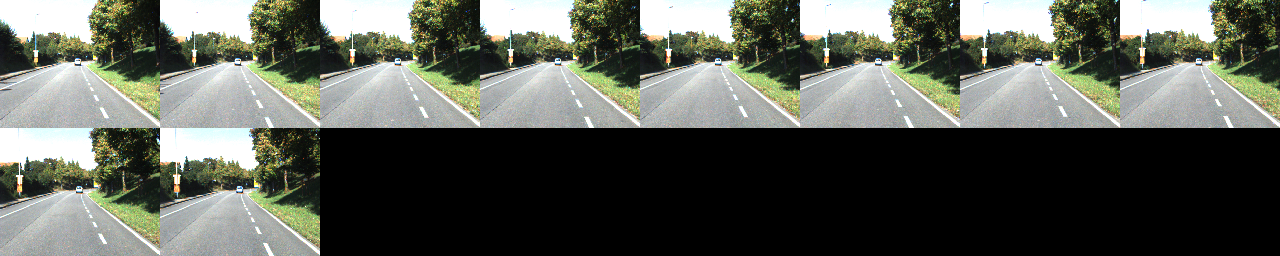
\includegraphics[width=0.7\textwidth]{../Images/prednet_kitti_groundtruth.png} }} 
   \qquad
   \subfloat[ConvLSTM]{{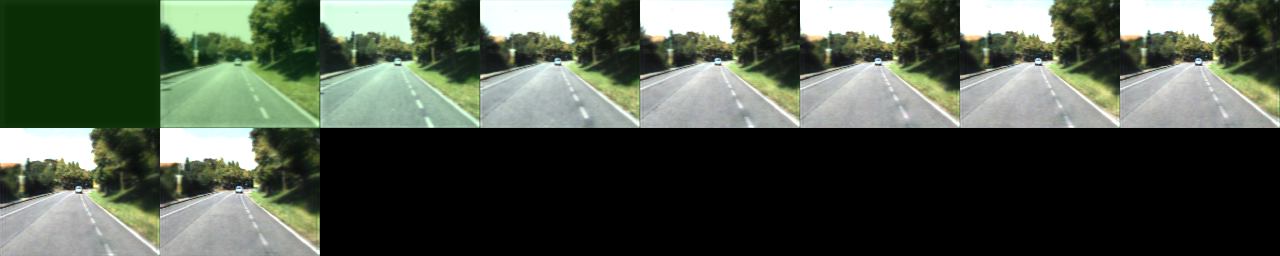
\includegraphics[width=0.7\textwidth]{../Images/prednet_kitti_convlstm.png} }} 
   \qquad
   \subfloat[PredRNN]{{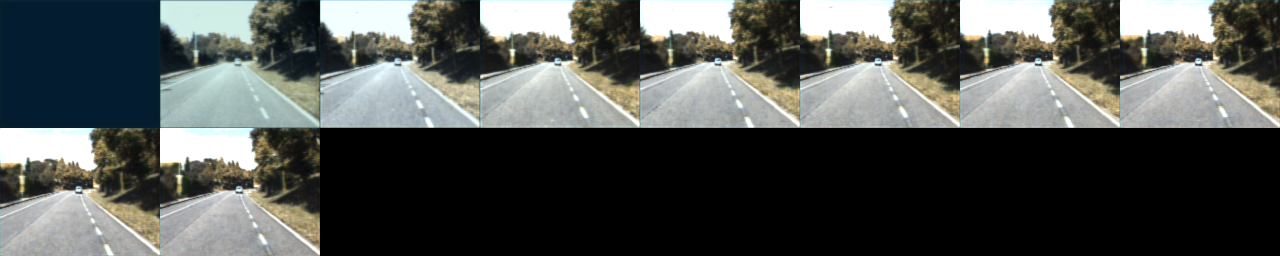
\includegraphics[width=0.7\textwidth]{../Images/prednet_kitti_predrnn.png} }}
   \caption{Test results for PredNet on Kitti.}
   \label{figure::prednet_kth_results}
  \end{figure}\noindent
   \begin{table}[H]
    \begin{center}
     \begin{tabular}{| l | l | l |}\hline
      \textbf{Model} & \textbf{ConvLSTM} & \textbf{PredRNN} \\\hline
      Autoencoder (Depth $2$) & $0.02$ & $0.013$ \\\hline
      PredNet & $0.019$ & $0.02$ \\\hline
      Spatiotemp & $0.018$ & $0.017$ \\\hline
     \end{tabular}
    \end{center}
    \caption{Mean MSE for Kitti.}
   \end{table}
 
 % discussion
 % section
\section{Discussion} \label{section::discussion}
 The related work showed, how differently state-of-the-art architectures for image-/video-prediction get to the same result, but also how they rely on the same
 recurrent module to achieve this results. It also showed how previous work in a field is used to adapt and overcome issues and reach better accuracy.\\
 In this example the paper from Shi et al. \cite{Shi2015}, where they used the previous published work from Srivastava et al. \cite{Srivastava2015}, but invented 
 a novel LSTM module, which used in the Autoencoder architecture outperforms the inital architecture. Both paper showed, how impressive the usage of an 
 Autoencoder architecture is for image-/video-prediction, so possibly Patraucean et al. \cite{Patraucean2015} decided therefore to use a ConvLSTM architecture and 
 an Autoencoder scheme, but additional brought optical flow into the research field, as well as the idea to split the sequence information into space and time. 
 Lotter et al. \cite{Lotter2016} showed, that a concept known from the neuroscience literature can be used in a slightly adapted way,
 using also a LSTM module, to let a neural network perform nearly the same way, a human beeing performs.\\There are several discussions regarding this paper, if
 the authors really re-modeled the idea of predictive coding, this is shortly discussed by Sinapayen and Noda \cite{Sinapayen2019} and very deeply by Rane et al. 
 \cite{Rane2019}. Wang et al. \cite{Wang2017} then invented a novel ConvLSTM module, which not only has temporal memory, but also a spatiotemporal memory.
 \\\\
 %
 The implementation of the networks showed, how important it is nowadays for a machine learning researcher to have a very good understanding of a variety of deep 
 learning frameworks, such as PyTorch \cite{Paszke2019}.\\During the implementation of the networks and the review of relevant sources,
 I read several code bases which
 were not written very comprehensive and adaptable and in several different deep learning frameworks, which sometimes differ very strongly.
 This might be, due to the reason that the code should only work for the researches themselves, the researches use the framework which they are most
 comfortable with and is therefore not described that well, but I believe that this should be done always, especially for people not working everyday with such a 
 programming language or deep learning framework.
 \\\\
 %
 The first experiments, were all hyperparameter were fixed, showed a problem, which is fundamental in machine learning, hyperparameter optimization. Looking at
 the results from the first experiments, one can clearly see, that changing the standard ConvLSTM module with the more advanced PredRNN module didn't
 showed any performance boost.\\In contrast, the change only increased the number of trainable parameter in the networks, which will lead to a worse performance
 of the network. Thinking about embedded systems, with only few resources per task, this is very important, even for neural networks, which are expensive during
 training, but cheap for execution. After performing hyperparameter optimization as last task of the experiments, a simple example already showed a performance
 boost of $> 40\%$. Seeing this results, it would be interesting to also perform hyperparamter optimization for all $18$ setups and perform the tests again to
 see the full results afterwars. This was not unfortunately not applicable due to the limited time of the bachelorthesis.
 
 % conclusion
 % section
\section{Conclusion} \label{section::conclusion}
 The thesis showed different approaches for image-/video-prediction and how important the choice of the recurrent sub-module is.
 First the reader got an extensive introduction
 about all necessary topics, which were necessary to fully understand the following chapters. Then the thesis gave a comprehensive related work part, in which
 five state-of-the-art image-/video-prediction algorithms are described, by showing the architecture and the results of the experiments of the synthetic dataset.
 This five architectures showed, how different the approaches are to perform image-/video-prediction, but also how similar the approaches are in form of
 having a similar recurrent module and using a type of autoencoder architecture.
 \\\\
 Because the implementation
 of the three baselines is a big part of this bachelor thesis, the implementation chapter describes how the code is structured and how to use the code, so any
 user (with minimal knowledge of PyTorch / neural networks) is able to use and possibly adapt the code for validating the performed experiments or even perform
 own further experiments. Then the reader gets the methodology, in which the way how the experiments are performed is described in-depth, so the reader will 
 understand the key-aspects of the experiments.
 \\\\
 The experimental results were given in the experiments section.
 The experiments showed, how important the right choice of a recurrent module is and also how important hyperparameter optimization is in training neural networks.
 The first experiments were performed using static settings for all network implementations. This experiments showed how important hyperparameter optimization
 is for training neural networks and for machine learning in general. Those experiments showed, that without using the \glqq best\grqq hyperparameter for each
 network, the choice of a more advanced recurrent module is not necessary.
 \\\\ 
 After performing hyperparameter optimization and using given \glqq optimal\grqq values 
 from the implemented papers, the experiment showed, that
 PredRNN is indeed the superior module and should be used in those implemented architectures. 
 Lastly, there is the discussion in which
 the reader gets an interpretation of the experimental results and how they affect image-/video-prediction neural networks.
 \\\\
 For future experiments, it would be awesome to see how the three networks perform in multi-frame prediction and if this leverages e.g. PredNet to have a much
 better steering wheel prediction, which could be used for autonomous driving.
 
 % Explanation of self written thesis
 Erklärung über das selbstständige Verfassen von \glqq Comparing different state-of-the-art solutions for image prediction using time-series analysis\grqq\\
Ich versichere hiermit, dass ich die vorstehende Bachelorarbeit selbständig verfasst und keine anderen als die angegebenen Hilfsmittel benutzt habe. Die Stellen der obigen Arbeit, die anderen Werken dem Wortlaut oder dem Sinn nach entnommen wurden, habe ich in jedem einzelnen Fall durch die Angabe der Quelle bzw. der Herkunft, auch der benutzten Sekundärliteratur, als Entlehnung kenntlich gemacht. Dies gilt auch für Zeichnungen, Skizzen, bildliche Darstellungen sowie für Quellen aus dem Internet und anderen elektronischen Text-und Datensammlungen und dergleichen. Die eingereichte Arbeit ist nicht anderweitig als Prüfungsleistung verwendet worden oder in deutscher oder in einer anderen Sprache als Veröffentlichung erschienen. Mir ist bewusst, dass wahrheitswidrige Angaben als Täuschung behandelt werden.\\\\
Datum, Ort Unterschrift\\ 
 
 % literature
% \newpage
% \pagestyle{empty}
 \pdfbookmark[section]{Bibliography}{Bibliography}
 \bibliography{../Bibliography/bibliography.bib} \label{section::literature}

\end{document} 
 
